\chapter{Overview of the Search of \texorpdfstring{\hmm}{H to Muons} Decay at CMS}\label{chp:hmm_overview}
% Need to use \textorpdfstring{} so it also shows in pdf bookmarks 

As described in Section~\ref{sec:SM_parameters}, the Yukawa couplings between the Higgs boson and the elementary fermions are essential parameters to the SM.
The Higgs couplings to fermions of the first and second generations are hard to probe because the Higgs boson decay ratios to these light fermions are small.
At the LHC, the most experimentally sensitive way to probe such light Yukawa couplings is the study of the \hmm decay.
Prior to this work, searches for the \hmm decay has been conducted using $pp$ collision data collected at center-of-mass energies of 7, 8, and 13 \TeV
by CMS~\cite{2015184, PhysRevLett.122.021801} and ATLAS~\cite{201468, PhysRevLett.119.051802, Aad:2020xfq},
among which the most sensitive result~\cite{PhysRevLett.122.021801} is reported by CMS with an observed (expected in absence of \hmm decay) upper limit of 2.9 (2.2) times the 
SM prediction of the Higgs boson production and \brhmm, at the 95\% confidence level (CL).
This thesis reports the latest \hmm analysis based on 137~\invfb of data collected by CMS from 2016 to 2018~\cite{Sirunyan_2021}.

The search for the \hmm decay, in a nutshell, is a struggle to make the signal events stand out from the vast backgrounds with statistical significance.
The \hmm decay has a branching ratio of ${\brhmm = 2.18 \times 10^{-4}}$, 
which corresponds to an expectation of about 1000 event instances in the data collected by CMS from 2016 to 2018.
In contrast, these 1000 signal events are accompanied by millions of events produced through other processes (background events) that mimic their experimental signature.
The most important difference between the signal events and the background events lies in the dimuon invariant mass (\mmm) distribution, illustrated in Figure~\ref{fig:dimuon_mass_shapes}.
The SM Higgs boson has a low production cross section and a narrow natural width, making a small sharp peak near 125~\GeV.
The background events are dominated by the $\PZ/\gamma^{*} \to \mu\mu$ process (Drell-Yan process), 
which peaks at 91.2~\GeV in the \mmm spectrum and leaves a smooth falling tail around 125~\GeV.
The overall signal-to-background ratio (\SoB) between 120 and 130~\GeV is about 1/500 in the 2016-2018 CMS data.

\begin{figure}[!htb]
    \centering
%    \captionsetup{justification=justified}
    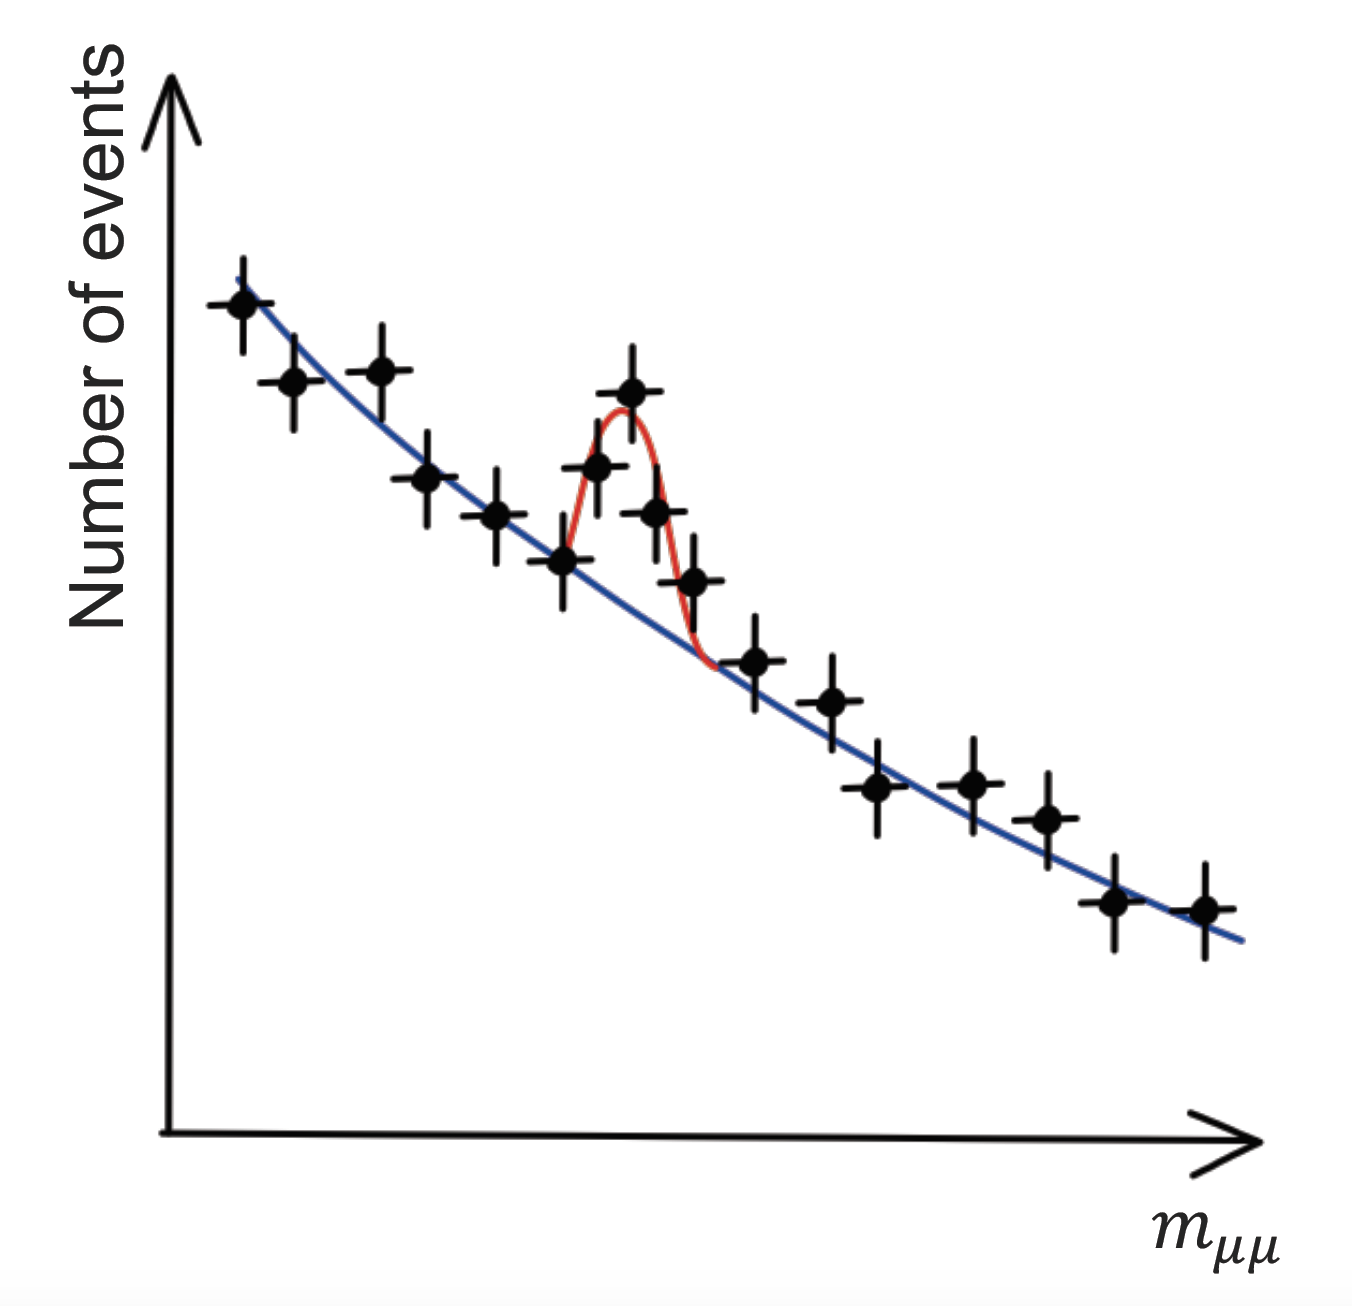
\includegraphics[width=0.6\textwidth]{pics/hmm_mass_sketch.png}
    \caption{A conceptual plot for the dimuon mass shapes for the signal and the background. 
             The blue line shows the expected background shape, while the red line shows the expected signal shape on top of it.}
    \label{fig:dimuon_mass_shapes}
\end{figure}

This \SoB can be enhanced based on further kinematic distinctions between various signal and background processes.
The Higgs boson is produced via several production modes.
The four main modes, ordered by their cross sections, are gluon fusion (\ggH), vector boson fusion (\qqH or qqH), 
associated production with a weak vector boson (\VH), and associated production with a pair of top quarks (\ttH). 
The Feynman diagrams for these main production modes are shown in Figure~\ref{fig:main_higgs_modes}.
The minor production modes include associated production with a pair of bottom quarks (\bbH),
associated production with a \PZ boson through gluon fusion (\ggZH), 
associated production with a top quark and a \PW boson (\tHW), 
and associated production with a top quark and a light quark (\tHq). 
The Feynman diagrams for these minor production modes are shown in Figure~\ref{fig:minor_higgs_modes}.
Table~\ref{tab:signal_xsec} summarizes the cross sections for all these production modes, 
along with the expected number of events in the 137~\invfb data.

\begin{figure}[!htb]
    \centering 
    \captionsetup{justification=centering}
    \begin{subfigure}[b]{0.45\textwidth} % b for bottom alignment so caption is at the same height
        \centering
        \feynmandiagram[horizontal=g1 to t1, horizontal=t2 to h] {
            g1 [particle = \Pg] -- [gluon] t1,
            t1 -- [fermion, edge label = \Pqt] t2 -- [fermion, edge label = \Pqt] t3 -- [fermion, edge label = \Pqt] t1,
            g2 [particle = \Pg] -- [gluon] t3,
            t2 -- [scalar] h [particle = \PH],
            g1 -- [draw=none] g2,
        };

        \caption*{\ggH}
    \end{subfigure} 
    %to put these two diagrams side by side. no empty line in between these two blocks, otherwise it indicates an empty line in the pdf
    \begin{subfigure}[b]{0.45\textwidth}
        \centering
        \feynmandiagram[horizontal=b to h]{
            q1 [particle = $\Pq_{1}$] -- [fermion] a -- [fermion] aq1 [particle = $\Pq^\prime_{1}$],
            a -- [boson, edge label = \PV] b -- [boson, edge label = \PV] c,
            b -- [scalar] h [particle = \PH],
            aq2 [particle = $\Pq_{2}$] -- [fermion] c -- [fermion] q2 [particle = $\Pq^\prime_{2}$],

            q1 -- [draw = none] n -- [draw = none] aq2,
            a -- [draw = none] c,
            aq1 -- [draw = none] h -- [draw = none] q2,

        };
        \caption*{\qqH}
    \end{subfigure}

    \begin{subfigure}[b]{0.45\textwidth}
        \centering
        \feynmandiagram[horizontal=a to b] {
            q [particle = \Pq] -- [fermion] a -- [anti fermion] aq [particle = $\Pq^\prime$],
            a -- [boson, edge label = \PV] b,
            v [particle = \PV] -- [boson] b -- [scalar] h [particle = \PH],
        };
        \caption*{\VH}
    \end{subfigure}
    \begin{subfigure}[b]{0.45\textwidth}
        \centering
        \feynmandiagram[horizontal=b to h]{
            g1 [particle = \Pg] -- [gluon] a -- [fermion] t1 [particle = \Pqt],
            a -- [anti fermion, edge label = \Paqt] b -- [anti fermion, edge label = \Pqt] c,
            b -- [scalar] h [particle = \PH],
            g2 [particle = \Pg] -- [gluon] c -- [anti fermion] t2 [particle = \Paqt],

            g1 -- [draw = none] n -- [draw = none] g2,
            a -- [draw = none] c,
            t1 -- [draw = none] h -- [draw = none] t2,
        };
        \caption*{\ttH}
    \end{subfigure}
    \caption{Main production modes of the Higgs boson.}
    \label{fig:main_higgs_modes}
\end{figure}



\begin{figure*}[!htb]
    \centering
    \captionsetup{justification=centering}
    \begin{subfigure}[b]{0.45\textwidth}
        \centering
        \feynmandiagram[horizontal=b to h]{
            g1 [particle = \Pg] -- [gluon] a -- [fermion] b1 [particle = \Pqb],
            a -- [anti fermion, edge label = \Paqb] b -- [anti fermion, edge label = \Pqb] c,
            b -- [scalar] h [particle = \PH],
            g2 [particle = \Pg] -- [gluon] c -- [anti fermion] b2 [particle = \Paqb],

            g1 -- [draw = none] n -- [draw = none] g2,
            a -- [draw = none] c,
            b1 -- [draw = none] h -- [draw = none] b2,
        };
        \caption*{\bbH}
    \end{subfigure}
    \begin{subfigure}[b]{0.45\textwidth}
        \centering
        \feynmandiagram[horizontal=a to b] {
            g [particle = \Pg] -- [gluon] a -- [anti fermion] qb [particle = \Pqb],
            a -- [fermion, edge label = \Pqb] b,
            w [particle = $\PW^{-}$] -- [boson] b -- [fermion, edge label = \Pqt] th -- [fermion] t [particle = \Pqt],
            th -- [scalar] h [particle = \PH],
            t -- [draw = none] h -- [draw = none] w, 
        };
        \caption*{\tHW}
    \end{subfigure}

    \begin{subfigure}[b]{0.45\textwidth}
        \centering
        \feynmandiagram[vertical=a to b] {
            q [particle = \Pq] -- [fermion] a -- [fermion] aq [particle = \Pq'],
            a -- [boson, edge label = \PW] b,
            qb [particle = \Pqb] -- [fermion] b -- [fermion, edge label = \Pqt] c,
            c -- [scalar] h [particle = \PH],
            c -- [fermion] t [particle = \Pqt],
            q -- [draw = none] n -- [draw = none] qb,
            aq -- [draw = none] h -- [draw = none] c,
            aq -- [draw = none] h -- [draw = none] t,
        };
        \caption*{\tHq}
    \end{subfigure}
    \begin{subfigure}[b]{0.45\textwidth}
        \centering
        \feynmandiagram[horizontal=b to h]{
            q1 [particle = \Pq] -- [fermion] a -- [fermion] q2 [particle = $\Pq^\prime$],
            a -- [boson, edge label = \PW] b -- [boson, edge label = \PW] c,
            b -- [scalar] h [particle = \PH],
            qb [particle = \Pqb] -- [fermion] c -- [fermion] qt [particle = \Pqt],

            q1 -- [draw = none] n -- [draw = none] qb,
            a -- [draw = none] c,
            q2 -- [draw = none] h -- [draw = none] qt,
        };
        \caption*{\tHq}
    \end{subfigure}

    \begin{subfigure}[b]{0.45\textwidth}
        \centering
        \feynmandiagram[horizontal=g1 to q1, horizontal=q2 to z] {
            g1 [particle = \Pg] -- [gluon] q1,
            q1 -- [fermion, edge label' = \Pq] q2 -- [fermion, edge label' = \Pq] q3 -- [fermion, edge label' = \Pq] q1,
            g2 [particle = \Pg] -- [gluon] q3,
            q2 -- [boson, edge label = \PZ] z ,
            z -- [boson] z2 [particle = \PZ],
            z -- [scalar] h [particle = \PH],
            g1 -- [draw=none] g2,
        };
        \caption*{\ggZH}
    \end{subfigure} 
    \begin{subfigure}[b]{0.45\textwidth}
        \centering
        \feynmandiagram[horizontal=t1 to t2] {
            g1 [particle = \Pg] -- [gluon] t1 -- [fermion, edge label = \Pqt] t2 -- [boson] z [particle = \PZ],
            g2 [particle = \Pg] -- [gluon] t4 -- [anti fermion, edge label = \Pqt] t3 -- [scalar] h [particle = \PH],
            t1 -- [anti fermion, edge label = \Pqt] t4,
            t2 -- [fermion, edge label = \Pqt] t3,
            g1 -- [draw = none] g2,
            z -- [draw = none] h,
        };
        \caption*{\ggZH}
    \end{subfigure} 
    \caption{Examples of minor Higgs boson production modes.}
    \label{fig:minor_higgs_modes}
\end{figure*}

\begin{table}[!htb]
    \centering
%    \captionsetup{justification=justified}
    \topcaption{Production modes of the Higgs boson in $pp$ collisions at the LHC, their cross sections for $\mh = 125 \GeV$, 
                and the corresponding expected number of \hmm decays in the dataset for this analysis 
                (the cross sections multiplying \brhmm and the integrated luminosity ($137 \invfb$). 
                The leptons ($\ell$) in the table refer to electrons or muons.}
    \begin{tabular}{lccc}
        \hline
        signal mode         & decay mode                & Cross section (\pb)   & Expected \hmm events \\
        \hline
        \ggH                & inclusive                 & 48.58                 & 1450 \\
        \qqH                & inclusive                 & 3.782                 & 113 \\
        \WH                 & inclusive                 & 1.373                 & 41.0 \\
                            & $\PW\to\ell\nu$           & 0.293                 & 8.75 \\
%                            & $\PW\to$ hadrons          & 0.926                 & 27.6 \\
        ${\Pq\Pq\to\PZ\PH}$ & inclusive                 & 0.761                 & 22.7 \\
                            & $\PZ\to\ell\ell$          & 0.051                 & 1.53 \\
%                            & $\PZ\to\nu\nu$            & -                     & - \\
%                            & $\PZ\to$ hadrons          & -                     & - \\
        \ggZH               & inclusive                 & 0.123                 & 3.67 \\
                            & $\PZ\to\ell\ell$          & 0.008                 & 0.25 \\
%                            & $\PZ\to\nu\nu$            & -                     & - \\
%                            & $\PZ\to$ hadrons          & -                     & - \\
        \ttH                & inclusive                 & 0.507                 & 15.1 \\
                            & $\geq 1~\Pqt\to$ leptons  & 0.193                 & 5.76 \\
                            & Both $\Pqt\to$ hadrons    & 0.230                 & 6.86 \\
        \hline
        sum of above        & inclusive                 & 55.13                 & 1646 \\
        \hline
        \bbH                & inclusive                 & 0.488                 & 14.6 \\
        \tHq                & inclusive                 & 0.074                 & 2.21 \\
        \tHW                & inclusive                 & 0.015                 & 0.45 \\
        \hline
        sum of all          & inclusive                 & 55.70                 & 1663 \\
        \hline
    \end{tabular}
    \label{tab:signal_xsec}
\end{table}

To fully exploit the kinematic profiles of different production modes, 
the \hmm analysis is performed in four event categories targeting each of the four main modes,
with the analysis procedures optimized separately in each category.
No dedicated category is made for the minor signal modes, 
either because they have very similar features to one of the main modes, 
or because their cross sections are too small to be statistically significant.
This chapter gives an overview of the full \hmm analysis, 
with Section~\ref{sec:data_mc_samples} describing the data and simulation samples used in the analysis, 
and Section~\ref{sec:hmm_cat_and_strategy} explaining the analysis strategies in the four exclusive categories.


\bigskip
\section{Data and Simulation Samples}\label{sec:data_mc_samples}

This analysis uses the $pp$ collision data collected by CMS from 2016 to 2018,
corresponding to an integrated luminosity of 137\invfb.
The triggers used in this analysis are the single muon HLT triggers, 
which impose some loose isolation requirements and a \pt threshold on the HLT muon candidates.
The \pt threshold is 24/27/24 \GeV for 2016/2017/2018 datasets.
The efficiencies of these triggers are above 90\% for single muons above the trigger thresholds,
and the overall efficiency for events with two muons is close to 100\%.

Simulations of signal and background processes are produced by Monte Carlo (MC) event generators.
The generators are listed for different processes in the rest of this section.
All simulated samples except the EW~$\PZ+jj$ samples use \PYTHIA 8.2~\cite{SJOSTRAND2015159} to model the parton showering (PS), 
hadronization, and the underlying event (UE), while the EW~$\PZ+jj$ samples use \HERWIGpp and \HERWIGSeven~\cite{Bellm:2015jjp} for the same purpose.
The effect of pileup is modeled by overlaying simulated inelastic $pp$ collisions on the hard-scattering event.
The generated events are processed through a simulation of the CMS detector based on \GEANTfour~\cite{AGOSTINELLI2003250}
and are reconstructed with the same algorithms that are used for data.

\bigskip
\subsection{Simulation of Signal Processes}
The \ggH signal process is simulated at next-to-leading order (NLO) accuracy in perturbative QCD, using both the \MGvATNLO~v2.4.2~\cite{Alwall:2014hca}
and \POWHEG~v2.0~\cite{Nason_2004, Frixione_2007, Alioli:2010xd, Bagnaschi:2011tu} event generators. 
The \pt distribution of the Higgs boson in \ggH process is then reweighted to match the \POWHEG~\textsc{nnlops} prediction~\cite{Hamilton:2013fea,Hamilton:2015nsa}. 
The \qqH, \WH, \qqZH, and \ttH processes are simulated with \POWHEG~v2.0~\cite{Nason:2009ai,Luisoni:2013kna,Hartanto:2015uka} at NLO precision in QCD. 
The \bbH process is simulated at NLO precision in QCD with \POWHEG.
the \tHq, and \tHW processes are generated at leading order (LO) with the \MGvATNLO generator.
The \ggZH process is simulated at LO with the \POWHEG generator.
Simulated signal events are generated, for each production mode, at \mh values of 120, 125, and 130~\GeV.
A table summarizing the simulation for signals is shown in Table~\ref{tab:sig_samples}.

\begin{table}[!htb]
    \centering
    \captionsetup{justification=centering}
    \topcaption{Summary of the specification for the simulated Higgs signal samples.}
    \resizebox{\textwidth}{!}{\begin{tabular}{lcccc}
        \hline
        Sample                 &Generator (Perturbative order)    &Parton Shower          &Cross section      &Additional corrections\\
        \hline
        \ggH                   &\MGvATNLO (NLO QCD)               &\PYTHIA                &N3LO QCD, NLO EW   &$\pt(\PH)$ from \textsc{nnlops}\\
        \qqH                   &\POWHEG (NLO QCD)                 &\PYTHIA dipole shower  &NNLO QCD, NLO EW   & -\\
        ${\Pq\Pq\to\PV\PH}$    &\POWHEG (NLO QCD)                 &\PYTHIA                &NNLO QCD, NLO EW   & -\\
        \ggZH                  &\POWHEG (LO)                      &\PYTHIA                &NNLO QCD, NLO EW   & -\\
        \ttH                   &\POWHEG (NLO QCD)                 &\PYTHIA                &NLO QCD, NLO EW    & -\\
        \bbH                   &\POWHEG (NLO QCD)                 &\PYTHIA                &NLO QCD            & -\\
        \tHq                   &\MGvATNLO (LO)                    &\PYTHIA                &NLO QCD            & -\\
        \tHW                   &\MGvATNLO (LO)                    &\PYTHIA                &NLO QCD            & -\\
        \hline
    \end{tabular}}
    \label{tab:sig_samples}
\end{table}

Expected signal yields are normalized to the production cross sections and \brhmm values taken from the recommendations of LHC Yellow Report~\cite{deFlorian:2016spz}.
The \ggH production cross section is computed at next-to-next-to-NLO (N3LO) precision in QCD, and at NLO in EW theory~\cite{Anastasiou:2016cez}. 
The cross section of Higgs boson production in the VBF~\cite{Cacciari:2015jma} and ${\Pq\Pq\to\PV\PH}$~\cite{Brein:2003wg} modes is calculated at next-to-NLO (NNLO) in QCD, 
including NLO EW corrections, while the \ttH cross section is computed at NLO in QCD and EW theory~\cite{Dawson:2003zu,Frixione:2014qaa}. 
The \bbH, \tHq, and \tHW cross sections are computed at NLO in QCD without including higher-order EW corrections~\cite{deFlorian:2016spz,Demartin:2015uha,Demartin:2016axk}. 
The \hmm partial width is computed with \textsc{hdecay}~\cite{Djouadi:1997yw,Spira:1997dg} at NLO in QCD and EW theory.

\bigskip
\subsection{Simulation of Background Processes}
The background is modeled considering various SM processes, summarized in Table~\ref{tab:bkg_samples}.
The main background in the \ggH and \qqH categories is the DY process, which is simulated at NLO in QCD using the \MGvATNLO generator. 
The corresponding cross section is calculated with \FEWZ~v3.1b2~\cite{Li:2012wna} at NNLO in QCD and NLO accuracy in EW theory. 
The EW production of a $\PZ$ boson in association with two jets ($\PZ+jj$) is an important background in the VBF category. 
This process is simulated at LO using the \MGvATNLO~v2.6.5 generator. 
The $\PW\PZ$, ${\Pq\Paq\to\PZ\PZ}$, and $\PW\PW$ processes, which constitute the main backgrounds in the $\PV\PH$ category, 
are simulated at NLO in QCD using either the \POWHEG or \MGvATNLO generators. 
Their production cross sections are corrected with the NNLO/NLO $K$ factors taken from Refs.~\cite{Grazzini:2017ckn},~\cite{Grazzini:2015hta}, and~\cite{Gehrmann:2014fva}. 
The gluon-initiated loop-induced ZZ process (\ggZZ) is simulated with the \MCFM~v7.0 generator~\cite{Campbell:2011bn} at LO 
and the corresponding production cross section is corrected to match higher-order QCD predictions, following the strategy detailed in Ref.~\cite{Sirunyan:2017exp}. 
Minor contributions from triboson processes ($\PW\PW\PW$, $\PW\PW\PZ$, $\PW\PZ\PZ$, and $\PZ\PZ\PZ$) are also taken into account and are simulated at NLO in QCD using the \MGvATNLO generator. 
The main backgrounds in the \ttH category involve the production of top quarks. 
The $\Pqt\Paqt$ background is simulated with NLO precision in QCD using the \POWHEG generator, and its cross section is obtained from the \TOPpp~v2.0~\cite{Czakon:2011xx} prediction 
that includes NNLO corrections in QCD and resummation of next-to-next-to-leading logarithmic (NNLL) soft gluon terms. 
The single top quark processes are simulated at NLO in QCD via either \POWHEG or \MGvATNLO and their cross sections are computed, 
at the same order of precision, using \textsc{hathor}~\cite{Kant:2014oha}. 
Finally, contributions from the $\Pqt\Paqt\PZ$, $\Pqt\Paqt\PW$, $\Pqt\Paqt\PW\PW$, ${\Pqt\Paqt\Pqt\Paqt}$, and \tZq processes 
are also considered and are simulated using the \MGvATNLO generator at NLO precision in QCD. 
For the simulated samples corresponding to the 2016 (2017--2018) data-taking periods, the NNPDF~v3.0~(v3.1) NLO (NNLO) parton distribution functions (PDFs) are used~\cite{Ball:2014uwa,Ball:2017nwa}. 
For processes simulated at NLO (LO) in QCD with the \MGvATNLO generator, events from the matrix element (ME) characterized by different parton multiplicities are merged via the FxFx (MLM) prescription~\cite{Alwall:2007fs,Frederix:2012ps}.


\begin{table}[!htb]
    \centering
    \captionsetup{justification=centering}
    \topcaption{Summary of the specification for the simulated background samples.}
    \resizebox{\textwidth}{!}{\begin{tabular}{lcccc}
        \hline
        Sample                              &Generator (Perturbative order)    &Parton Shower          &Cross section      &Additional corrections\\
        \hline
        Drell-Yan                           &\MGvATNLO (NLO QCD)               &\PYTHIA                &NNLO QCD, NLO EW   & -\\
        Zjj-EW                              &\MGvATNLO (LO)                    &\HERWIGpp/\HERWIGSeven &LO                 & -\\
        $\Pqt\Paqt$                         &\POWHEG (NLO QCD)                 &\PYTHIA                &NNLO QCD           & -\\
        Single top quark                    &\POWHEG/\MGvATNLO (NLO QCD)       &\PYTHIA                &NLO QCD            & -\\
        Diboson ($\PV\PV$)                  &\POWHEG/\MGvATNLO (NLO QCD)       &\PYTHIA                &NLO QCD            & NNLO/NLO $K$ factors\\
        \ggZZ                               &\MCFM (LO)                        &\PYTHIA                &LO                 & NNLO/LO $K$ factors\\
        $\Pqt\Paqt\PV$, $\Pqt\Paqt\PV\PV$   &\MGvATNLO (NLO QCD)               &\PYTHIA                &NLO QCD            & -\\
        Triboson ($\PV\PV\PV$)              &\MGvATNLO (LO)                    &\PYTHIA                &NLO QCD            & -\\
        \hline
    \end{tabular}}
    \label{tab:bkg_samples}
\end{table}


\bigskip
\section{Exclusive Analyses and Their Strategies}\label{sec:hmm_cat_and_strategy}

The \hmm analysis is conducted independently in four event categories: the \ggH, \qqH, \VH and \ttH categories.
The workflow to divide events into these categories is shown in Figure~\ref{fig:event_categories}.
A prerequisite for all categories, after the trigger selection, 
is that each events should contain two opposite-charged (or opposite-sign, OS) muons that make the candidate for the Higgs boson decay. 
Then, as a first step, events containing b-tagged jets (either one medium tag or two loose tag of the DeepCSV~\cite{Sirunyan:2017ezt} working points) are classified into the \ttH category.
Events in the \ttH category are further divided into the \ttH leptonic subcategory if they contain electrons or additional muons,
or divided into the \ttH hadronic subcategory if they contain at least three jets,
or discarded if they contain neither of them.
The events without b-tagged jets may fall into the \VH category if they contain additional leptons (electrons or muons).
Inside the \VH category, events are further tagged as \WH events if there is one and only one extra lepton in the event, 
or tagged as \ZH events if there are two same-flavor opposite-sign (SFOS) extra leptons.
For the events with neither b-tagged jets nor additional leptons, 
if they have at least two energetic jets composing a jet pair with $\mjj > 400~\GeV$ and $\detajj > 2.5$, 
they are tagged as the \qqH events.
Finally, the \ggH category collects all events that are not assigned to other categories. 
The definitions of the different objects used in this categorization is detailed in Section~\ref{sec:obj_sel}.

\begin{figure}[!htb]
    \centering
%    \captionsetup{justification=justified}
    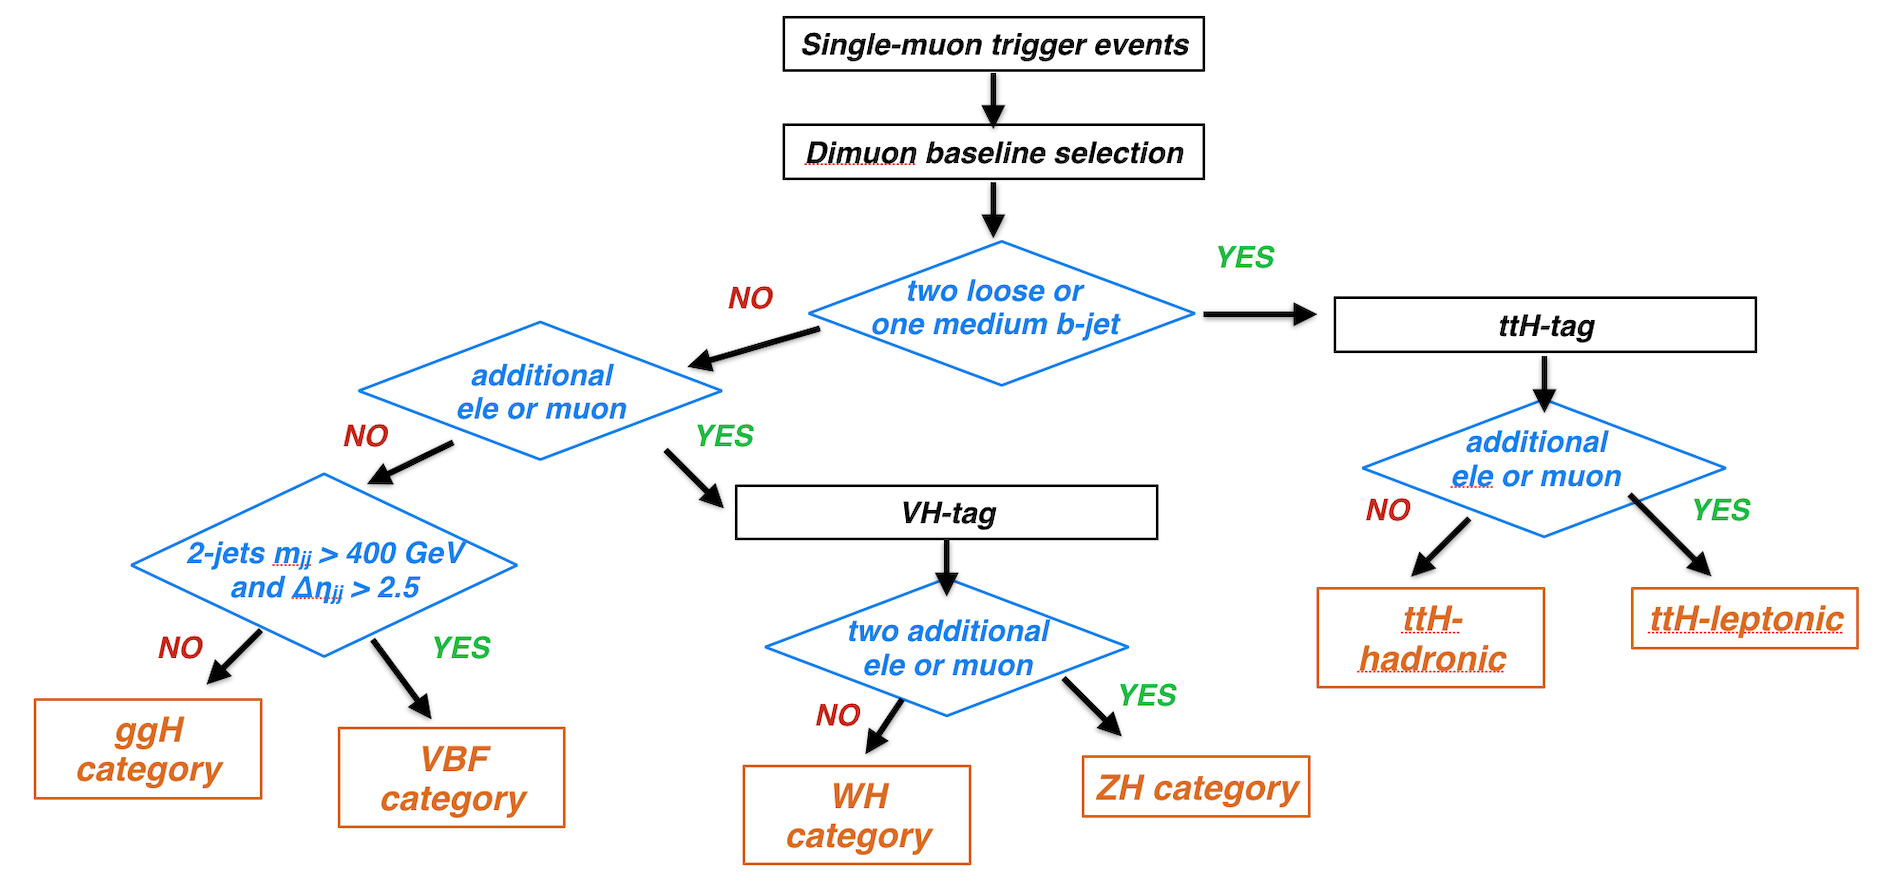
\includegraphics[width=0.9\textwidth]{pics/category_scheme.png}
    \caption{Scheme of the procedure of assigning events to different categories. All events passing the common baseline selection
             are divided into four mutually exclusive categories: \ggH, \qqH, \VH (\WH and \ZH), and \ttH (leptonic and hadronic).}
    \label{fig:event_categories}
\end{figure}

These categories have distinct profiles in expected signal yield, signal purity, and background composition.
Therefore the optimal analysis strategies are different.
Two strategies are considered for these categories:

\begin{itemize}
    \item \textbf{Data-driven parametric fit to the \mmm spectrum:} 
          As is done in the previously published analyses on the the data collected prior to 2017~\cite{2015184, PhysRevLett.122.021801},  
          a multivariate analysis (MVA) method is used to profile the separation between the signal and the background processes. 
          The MVA can be either cut-based as in the Run 1 analysis~\cite{2015184}, or machine learning (ML) based as in the analysis on the 2016 data~\cite{PhysRevLett.122.021801}.
          The MVA considers the kinematic information that is uncorrelated with the \mmm, and is used to divide the events into several regions 
          with different \SoB, called the MVA-categories. 
          In each MVA-category, the signal strength is evaluated from fits to the \mmm spectrum in data, in what is called the \textit{signal fit region}, for example $110<\mmm<150~\GeV$.
          Both the signal and the background are modeled by parametric functions that are carefully studied to provide a truthful description of the distributions of physics processes. 
          The total yield of the background is unconstrained in the fit and is determined entirely by the data.
          The effects of the systematic uncertainties from various sources on either the signal yield or the signal shape are assessed and propagated to the fit result. 
          The systematic uncertainties do not affect the background estimation since it is based on data rather than predictions from simulations.
    \item \textbf{MC-based template fit to the Neural Network discriminator:}
          This approach is also based on an MVA, for which a ML algorithm, Deep Neural Network (DNN), is taken.
          The DNN takes all the kinematic variables \textit{including \mmm}, and profiles the discrimination between the signal and the background.
          Without making further categories, the binned template of the DNN output in the whole phase space is used for the signal strength evaluation.
          Since the fit is applied to the DNN output rather than the \mmm distribution, the \textit{signal fit region} is further divided into two parts:
          the \textit{signal region}, $115<\mmm<135 ~\GeV$, and the \textit{sideband region}, $110<\mmm<115 ~\GeV$ or $135<\mmm<150 ~\GeV$.
          The data are fit simultaneously in both regions using the DNN templates of the signal and background simulation. 
          The systematic uncertainties affect both the signal and the background prediction, and are employed as variations in either the yield or the shape of the templates.
          The background yield is estimated from simulation and is allowed to vary within its uncertainty in the fit, in the same manner as the other systematic uncertainties.
          The signal strength is extracted from the fit in the \textit{signal region}.
          The \textit{sideband region} does not contain any signal contribution, but is nonetheless used in the fit, to enhance the constraint on the background estimation.
\end{itemize}

These two strategies should give comparable results in the ideal case, where there are abundant statistics in both data and simulation,
and where the data are well described by simulation.
However these conditions are usually not met in real analyses, and one strategy becomes preferable.
In scenarios where simulations do not model data very well, or where the uncertainties from simulations are not much smaller than the statistical uncertainty in data,
it is more advantageous to follow the data-driven approach.
In contrast, if an analysis lacks enough statistics in data but has abundant simulations that model data well, 
it is more beneficial to perform a MC-based analysis.

The \ggH category contains the majority of \hmm events with a very low \SoB. 
The statistical uncertainty of data is smaller than the systematic uncertainties of the background prediction from simulations.
Therefore it takes the data-driven strategy.
The \qqH category has a good amount of events, although much less than the \ggH category, and a good \SoB.
This makes it possible to pick very high \SoB regions with the help of MVA discriminators. 
The \qqH analysis prefers the MC-based strategy as there may be too few events in the high \SoB regions for a data-driven analysis.
The \VH and \ttH categories both have very few events, but high \SoB, which seem like good playgrounds for the MC-based approach.
However, the main backgrounds in the \VH and \ttH categories involve extra lepton(s) from nonprompt sources, which lacks accurate simulation estimates.
Moreover, the \VH and \ttH categories have less sensitivity than the \ggH and \qqH categories.
Adopting the MC-based approach in the \VH and \ttH categories would take a lot of computation resources and lead to insignificant improvements to the overall result.
The data-driven approach is much more cost-effective in the \VH and \ttH categories.
Overall, the \ggH, \VH, and \ttH categories follow the data-driven strategy, while the \qqH category takes the MC-based approach.

This thesis is focused on the analysis in the \VH category, the procedures of which are detailed in Chapter~\ref{chp:VH_analysis}.
The summary of all categories is reported in Ref.~\cite{Sirunyan_2021}.
Chapter~\ref{chp:hmm_results} describes the results of the \VH analysis and the combined results of all four categories.
